\documentclass[conference]{IEEEtran}
\IEEEoverridecommandlockouts
\usepackage[OT1]{fontenc}
\usepackage{cite}
\usepackage{amsmath,amssymb}
\usepackage{graphicx}
\usepackage{booktabs}
\usepackage{multirow}
\usepackage{xcolor}
\usepackage{tikz}
\usetikzlibrary{arrows.meta,positioning}
\usepackage{url}
\usepackage[colorlinks=true,citecolor=blue,linkcolor=blue,urlcolor=blue]{hyperref}

\renewcommand{\citeleft}{\textcolor{blue}{[}}
\renewcommand{\citeright}{\textcolor{blue}{]}}
\newcommand{\cond}[1]{\texttt{#1}}

\begin{document}

\title{OmniEyes: Early-Layer Similarity Gating for Frame Selection in Streaming Omnimodal Assistants}

\author{
\IEEEauthorblockN{Aryan Rao, Saksham Agarwal, Shiva P, Mohammad Zaid Agha, Kavya Paras Shah, Soumitra Ashish Kulkarni}
\IEEEauthorblockA{BITS F471 Introduction to Large Language Models, Group 9\\
Birla Institute of Technology and Science, Pilani, K K Birla Goa Campus, India}
}

\maketitle

\begin{abstract}
Streaming omnimodal assistants can spend substantial computation encoding near-duplicate video frames. OmniEyes uses cosine similarity between corresponding patch features from the first three vision transformer blocks to choose which frames to encode fully. We evaluate Qwen2.5-Omni-3B on causal windows from 150 PhoStream questions across 13 selection conditions and two audio configurations (3{,}900 question-condition evaluations). With audio at the 0.88 threshold, the gate reduces the mean number of fully encoded frames from 32.5 to 14.0, prompt tokens from 3{,}254 to 1{,}675 (49\%), and reported time per question by 41\%. The mean natural-language inference (NLI) score falls from 26.9 to 25.4 (difference $-1.5$ points, 95\% bootstrap confidence interval $[-10.1,7.0]$). This interval leaves performance retention inconclusive. Without audio, three of four gate thresholds show statistically detectable losses relative to the unpruned reference. With audio, the gate takes more time than matched-budget uniform and pixel-difference selectors and shows no statistically detectable score advantage over either.
\end{abstract}

\begin{IEEEkeywords}
early exit, efficient inference, frame selection, omnimodal models, streaming video understanding, vision transformer
\end{IEEEkeywords}

\section{Introduction}
Omnimodal models such as GPT-4o~\cite{openai2024gpt4o}, Qwen2.5-Omni~\cite{xu2025qwen25omni} and Qwen3-Omni~\cite{xu2025qwen3omni} process text, images, audio and video in one network, which makes a continuously listening and watching phone assistant technically possible. In such a stream, however, the expensive step is visual: every frame is encoded by a deep vision transformer (ViT)~\cite{dosovitskiy2021vit} and becomes hundreds of tokens in the language model's prompt, while consecutive frames from a phone camera are mostly redundant. The PhoStream benchmark~\cite{lu2026phostream} shows that mobile streaming is a distinct and under-measured regime: models must answer about what is on screen \emph{now} or a few seconds ago, from a continuous audio-visual stream.

Existing efficiency methods leave a gap for this setting. FastV~\cite{chen2024fastv}, IVTP~\cite{huang2024ivtp} and PruneVid~\cite{huang2024prunevid} reduce visual token counts at different stages of processing. Streaming memories such as VideoChat-Online~\cite{huang2025ovbench} compress history online, but still fully encode every frame before deciding what to keep. Embodied streaming systems~\cite{wang2026ellsa,liu2025vitae} sidestep the cost with fixed, short visual windows.

\textbf{Problem.} We ask whether early-layer feature similarity in a ViT can serve as a temporal gate that decides, \emph{before} deep encoding, which frames of a continuous stream are worth sending to an omni model, reducing computation while preserving answer quality on questions about recent visual events, and whether such a gate selects better frames than simply sampling fewer.

\textbf{Contributions.}
\begin{itemize}
\item \textbf{OmniEyes}, a training-free gate that runs only the first three ViT blocks of a frozen omni model on each frame and keeps frames whose features change, with two additional constraints: retain the newest frame and enforce a minimum frame budget.
\item A controlled evaluation on PhoStream with Qwen2.5-Omni-3B: 150 questions $\times$ 13 selection conditions $\times$ 2 audio configurations (3{,}900 evaluations), against \emph{matched-budget} uniform and pixel-difference baselines, with paired bootstrap confidence intervals.
\item A quantitative cost analysis of the gate's per-frame overhead, prompt savings and runtime trade-offs.
\item A local, API-free answer grader based on natural-language inference (NLI), validated against hand labels, and a record of the filename-collision diagnosis and dataset integrity checks.
\end{itemize}

\section{Related Work}
\subsection{Omnimodal foundation models}
GPT-4o~\cite{openai2024gpt4o} established end-to-end training across text, vision and audio. Open models followed: Qwen2.5-Omni~\cite{xu2025qwen25omni} streams audio and video through incrementally consuming encoders and aligns them in time with a shared positional scheme; Qwen3-Omni~\cite{xu2025qwen3omni} reports no unimodal degradation relative to same-size single-modality models; Ming-Flash-Omni~\cite{inclusionai2025mingflash} lowers per-token cost with a sparse mixture of experts (about 6.1B of 100B parameters active); and Stream-Omni~\cite{zhang2025streamomni} aligns vision and speech to the language backbone by their semantic relationships instead of plain concatenation. These models make the perceptual substrate available, and their visual encoders process the frames selected for input.

\subsection{Visual token pruning}
FastV~\cite{chen2024fastv} observes that deep large language model (LLM) layers pay little attention to image tokens and drops half of them after layer 2, saving about 45\% of FLOPs for LLaVA-1.5-13B with little accuracy loss. IVTP~\cite{huang2024ivtp} prunes tokens inside the vision encoder by attention rollout and inside the LLM with an instruction-derived pseudo-token, removing 88.9\% of visual tokens for a 1.0\% average accuracy drop. PruneVid~\cite{huang2024prunevid} merges static and spatially similar tokens in video and then prunes by question-to-video attention, keeping about 16\% of tokens. These methods reduce token counts within or after encoding. OmniEyes instead selects whole frames over time using early encoder representations.

\subsection{Streaming memory and frame selection}
VideoChat-Online~\cite{huang2025ovbench} processes live video with a pyramid memory that evicts the more redundant of two adjacent frames by cosine similarity and down-samples older frames, bounding the visual context to 832 tokens; replacing similarity-based eviction with first-in-first-out lowers its accuracy, which supports change-based selection. Its decisions are made after full encoding. ELLSA~\cite{wang2026ellsa} and VITA-E~\cite{liu2025vitae}, which see, hear, speak and act concurrently, instead fix the visual budget by design (one frame per one-second block with two seconds of history, and a single $224{\times}224$ frame, respectively). OmniEyes moves the keep-or-drop decision into the first blocks of the encoder, so dropped frames never pay for the deep layers, and selects frames independently of question content.

\subsection{Benchmarks for streaming assistants}
PhoStream~\cite{lu2026phostream} evaluates omni models as mobile assistants on continuous audio-visual streams with \emph{instant}, \emph{backward} and \emph{forward} questions. It reports that removing audio lowers accuracy on instant and backward questions, and that models answer forward questions prematurely. It measures accuracy only, not compute, which leaves open how much of a stream's visual input a model actually needs.

\section{Problem Formulation}\label{sec:formulation}
Let a video stream deliver frames $x_t$ and audio $a_t$. A question $q$ is asked at time $t_q$ with reference answer $y$. The assistant may use only the causal window $\mathcal{W}=[t_q-W,\,t_q]$ ($W{=}16$\,s), sampled at 2\,Hz, giving frames $x_1,\dots,x_N$ ($N\approx33$, $x_N$ is the newest) and the audio $a_{\mathcal{W}}$.

\textbf{Gate features.} Let $f^{(1:K)}$ denote the first $K$ of the $L$ blocks of the vision encoder ($L{=}32$, $K{=}3$). For each frame, $z_i=f^{(1:K)}(x_i)\in\mathbb{R}^{P\times d}$ are its $P$ patch-token features. The similarity of two frames is the mean per-token cosine similarity
\begin{equation}
s(z_i,z_j)=\frac{1}{P}\sum_{p=1}^{P}\frac{z_{i,p}^{\top}z_{j,p}}{\lVert z_{i,p}\rVert\,\lVert z_{j,p}\rVert}.
\end{equation}

\textbf{Selection.} A threshold $\tau$ defines a greedy, causal selection $S_\tau$: frame 1 is kept, and frame $i$ is kept if $s(z_i,z_{r})<\tau$, where $r$ is the last kept frame. The greedy stage can run incrementally. Two rules complete selection over the current window at question time: the newest frame $N$ is always kept, and if $|S_\tau|<m$ ($m{=}4$), frames are added one at a time by farthest-point selection, $\arg\min_{i\notin S}\max_{j\in S}s(z_i,z_j)$.

\textbf{Cost.} With $c_K$ the cost of blocks $1..K$ for one frame, $c_{\text{full}}$ that of a complete encoder pass and $c_{\text{res}}$ that of blocks $K{+}1..L$, the vision cost of a selection $S$ is
\begin{equation}\label{eq:cost}
C_{\text{vis}}(S)=N\,c_K+|S|\,c_{\text{full}}\quad\text{(ideal: } N\,c_K+|S|\,c_{\text{res}}),
\end{equation}
where the ideal form assumes kept frames resume from block $K$. Language-model cost grows with the prompt length, which is proportional to $|S|$ plus the fixed audio and text tokens. Uniform and pixel baselines with $|S|$ frames cost $|S|\,c_{\text{full}}$.

\textbf{Objective.} With $A(S)$ the NLI score of the answer produced from $S$, we seek
\begin{equation}
\min_{\tau}\ \mathbb{E}[C(S_\tau)]\quad\text{s.t.}\quad \mathbb{E}[A(S_\tau)]\ \ge\ \mathbb{E}[A(\{1..N\})]-\epsilon.
\end{equation}
Here $C$ is total inference cost and $\epsilon$ is a conceptual tolerance in score points. The experiments did not specify a noninferiority margin. We ask whether the gate reduces cost relative to full input (\textbf{H1}), retains answer quality (\textbf{H2}), and improves answer quality over matched-budget uniform or pixel-difference selection (\textbf{H3}).

\section{Methodology}
\subsection{Dataset}
We use PhoStream~\cite{lu2026phostream} from Hugging Face~\cite{phostream_hf}: 578 phone videos from four sources (screen-recorded tutorials, YouTube vlogs, recordings and the egocentric EgoBlind set). Of 2{,}770 instant and backward questions, 2{,}761 have their video in the release. We sample 150 with a fixed seed (101 instant, 49 backward, from 114 videos). Forward questions are excluded: their answer occurs after $t_q$, outside any causal window.

\begin{figure}[t]
\centering
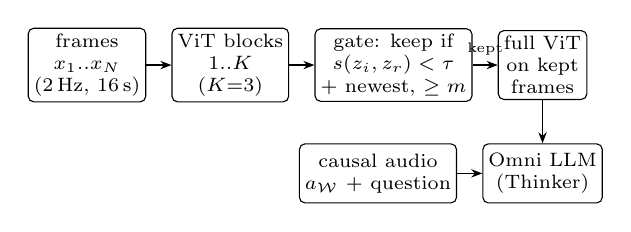
\begin{tikzpicture}[font=\scriptsize, node distance=0.35cm and 0.32cm,
  box/.style={draw, rounded corners=2pt, align=center, minimum height=0.75cm, inner sep=2pt},
  >={Stealth[length=4pt]}]
\node[box] (f) {frames\\$x_1..x_N$\\(2\,Hz, 16\,s)};
\node[box, right=of f] (k) {ViT blocks\\$1..K$\\($K{=}3$)};
\node[box, right=of k] (g) {gate: keep if\\$s(z_i,z_r)<\tau$\\+ newest, $\ge m$};
\node[box, right=of g] (v) {full ViT\\on kept\\frames};
\node[box, below=0.55cm of v] (l) {Omni LLM\\(Thinker)};
\node[box, left=of l] (a) {causal audio\\$a_{\mathcal{W}}$ + question};
\draw[->] (f) -- (k); \draw[->] (k) -- (g); \draw[->] (g) -- node[above, font=\tiny]{kept} (v); \draw[->] (v) -- (l); \draw[->] (a) -- (l);
\end{tikzpicture}
\caption{OmniEyes. Every frame first passes through $K$ encoder blocks. Kept frames are re-encoded in full and sent to the language model, with causal audio when enabled.}
\label{fig:pipeline}
\end{figure}

\subsection{Gate and selection}
The gate (Fig.~\ref{fig:pipeline}) attaches to the frozen vision encoder of Qwen2.5-Omni, which follows the Qwen2.5-VL design~\cite{bai2025qwen25vl} (32 blocks, mostly windowed attention). An early-exit hook stops the forward pass after block 3 and returns the patch features; selection follows Section~\ref{sec:formulation} with $\tau\in\{0.88,0.90,0.93,0.95\}$. The newest-frame rule and the 4-frame minimum were added after our first iterations, where the plain greedy rule kept only the oldest frame in 30--40\% of windows, so the model never saw the moment being asked about, and gate, uniform and pixel sampling degenerated to the same single frame.

\subsection{Answering model}
Kept frames, with their timestamps in the prompt, are given to the Thinker (text-generating part) of Qwen2.5-Omni-3B~\cite{xu2025qwen25omni} together with the audio of the same 16\,s window, which is never gated and never extends past $t_q$. Decoding is greedy with at most 64 new tokens, and the prompt asks for a direct, concise answer.

\subsection{Conditions and baselines}
Each question is answered 13 times: \cond{full} (all frames, the unpruned reference), and for each $\tau$, \cond{gate@$\tau$}, \cond{uniform@$\tau$} (the same number of frames, evenly spaced) and \cond{pixel@$\tau$} (the same number, chosen by largest mean pixel change). Both baselines also always include the newest frame. Matching the frame count isolates \emph{which} frames are chosen from \emph{how many}. With and without audio, this design comprises 3{,}900 evaluations across the same 150 questions.

\subsection{Grading and statistics}
API cost, rate limits and uninformative scores in an initial trial motivated local grading with an NLI model, DeBERTa-v3-large~\cite{he2023debertav3} fine-tuned for NLI~\cite{laurer2022nli}, with the reference as premise and the answer as hypothesis. The grade is $\text{ent\_con}=P(\text{entail})-P(\text{contradict})$, reported $\times100$ (from $-100$ to $+100$). We compare conditions with paired bootstrap 95\% confidence intervals~\cite{efron1993bootstrap} over the same questions (2{,}000 resamples). The intervals are unadjusted for multiple comparisons. Questions from the same video may be correlated, which question-level resampling does not account for. Isolated significant comparisons are exploratory.

\subsection{Implementation Details}
Two earlier iterations used Qwen2-VL-2B~\cite{wang2024qwen2vl} without audio, and built the grader and the cost accounting. Relative to our proposal, frames are sampled at 2\,Hz rather than 5\,Hz, the gate is a Python forward hook rather than a C++ wrapper, and kept frames are re-encoded from block 1 rather than resumed from block $K$; we report both actual and ideal (resumed) vision cost. Reported time combines synchronized wall-clock generation with a separate vision-cost estimate based on measured per-frame encoder times. The notebook starts the generation timer after input preparation and device transfer, and stops it before text postprocessing. Generation can include in-model visual and audio encoding, so the combined index is not an independent end-to-end wall-clock measurement. All models run in Hugging Face Transformers~\cite{wolf2020transformers} on a single T4 GPU in fp16.

\section{Experiments, Results and Discussion}
\subsection{Main results}

\begin{table}[t]
\centering
\caption{Mean NLI scores on 150 questions. Frames are fully encoded counts. Vision cost is estimated relative to encoding all frames. Vision estimates, tokens and times are for audio-enabled runs. Dashes mark unreported values.}
\label{tab:main}
\footnotesize
\setlength{\tabcolsep}{2.4pt}
\begin{tabular}{@{}lrrrrrr@{}}
\toprule
 & \multicolumn{2}{c}{NLI score} & & & & \\
\cmidrule(lr){2-3}
Condition & Audio & No audio & Frames & Vision & Tokens & Sec. \\
\midrule
\cond{full}          & \textbf{26.9} & \textbf{19.9} & 32.5 & 100\% & 3254 & 6.46 \\
\midrule
\cond{gate@0.88}     & \textbf{25.4} & 12.5 & 14.0 & 58\% & 1675 & 3.82 \\
\cond{uniform@0.88}  & 20.1 & $-$0.4 & 14.0 & 43\% & 1675 & 3.34 \\
\cond{pixel@0.88}    & 23.3 & 7.3  & 14.0 & 43\% & 1675 & 3.33 \\
\midrule
\cond{gate@0.90}     & 23.8 & 6.5  & 15.9 & 64\% & 1835 & 4.12 \\
\cond{uniform@0.90}  & 19.9 & 2.5  & 15.9 & 49\% & -- & -- \\
\cond{pixel@0.90}    & 21.5 & 7.5  & 15.9 & 49\% & -- & -- \\
\midrule
\cond{gate@0.93}     & 23.2 & 6.0  & 19.0 & 74\% & 2102 & 4.65 \\
\cond{uniform@0.93}  & 20.6 & 11.1 & 19.0 & 58\% & -- & -- \\
\cond{pixel@0.93}    & 20.4 & 13.0 & 19.0 & 58\% & -- & -- \\
\midrule
\cond{gate@0.95}     & 22.3 & 11.6 & 21.6 & 82\% & 2322 & 5.09 \\
\cond{uniform@0.95}  & 20.9 & 9.4  & 21.6 & 66\% & -- & -- \\
\cond{pixel@0.95}    & 20.6 & 9.7  & 21.6 & 66\% & -- & -- \\
\bottomrule
\end{tabular}
\end{table}

\begin{table}[t]
\centering
\caption{Paired differences, gate $-$ baseline, mean [95\% bootstrap CI]. Bold estimates have intervals that exclude zero.}
\label{tab:paired}
\footnotesize
\setlength{\tabcolsep}{2.3pt}
\begin{tabular}{@{}llccc@{}}
\toprule
 & $\tau$ & vs.\ \cond{full} & vs.\ uniform & vs.\ pixel \\
\midrule
\multirow{4}{*}{\rotatebox{90}{audio}}
 & 0.88 & $-1.5$ [$-10.1$, 7.0] & $+5.3$ [$-2.7$, 13.0] & $+2.1$ [$-4.3$, 7.9] \\
 & 0.90 & $-3.2$ [$-10.7$, 4.7] & $+3.9$ [$-2.6$, 10.6] & $+2.3$ [$-4.2$, 8.5] \\
 & 0.93 & $-3.7$ [$-11.6$, 4.0] & $+2.6$ [$-5.9$, 11.0] & $+2.8$ [$-2.5$, 8.2] \\
 & 0.95 & $-4.6$ [$-11.5$, 2.0] & $+1.5$ [$-3.6$, 6.8] & $+1.7$ [$-2.1$, 5.8] \\
\midrule
\multirow{4}{*}{\rotatebox{90}{no audio}}
 & 0.88 & $-7.4$ [$-17.2$, 2.3] & $\mathbf{+12.8}$ [3.8, 22.6] & $+5.2$ [$-2.4$, 12.9] \\
 & 0.90 & $\mathbf{-13.4}$ [$-22.1$, $-4.7$] & $+4.0$ [$-4.1$, 12.7] & $-1.0$ [$-8.4$, 6.2] \\
 & 0.93 & $\mathbf{-13.9}$ [$-22.5$, $-6.4$] & $-5.1$ [$-13.3$, 2.8] & $-7.0$ [$-14.3$, 0.3] \\
 & 0.95 & $\mathbf{-8.3}$ [$-16.0$, $-0.9$] & $+2.3$ [$-7.0$, 11.5] & $+2.2$ [$-2.8$, 7.9] \\
\bottomrule
\end{tabular}
\end{table}

Table~\ref{tab:main} gives the main results and Table~\ref{tab:paired} the paired comparisons. The gate is adaptive: at $\tau{=}0.88$ it keeps the 4-frame minimum on 49 of 150 static windows (mostly screen recordings) and all frames on 7 windows with fast camera motion, 14.0 frames on average. Per frame, the gate's three blocks cost 14.8\,ms against 95.2\,ms for a full encoder pass (16\%).

\textbf{H1 (cost): supported against \cond{full}.} At $\tau{=}0.88$ the gate sends 57\% fewer frames, halves the prompt tokens (3{,}254 to 1{,}675), cuts model generation time from 3.37\,s to 2.01\,s and reported time per question by 41\% (6.46\,s to 3.82\,s). Its vision cost, however, is 58\% of \cond{full} against 43\% for uniform or pixel sampling at the same frame count, 1.2--1.4$\times$ higher across $\tau$, because every frame pays for blocks 1--3, including the dropped ones. At this threshold the gate takes 14.4\% and 14.7\% longer than the uniform and pixel baselines, respectively. Equation~\eqref{eq:cost} estimates a resumed vision cost of 51.8\% of full encoding from the logged mean counts and reported per-frame timings. This estimate assumes reuse of block-3 features, which the implementation does not perform.

\textbf{H2 (answer quality): inconclusive with audio.} With audio, no gate setting is significantly worse than \cond{full} ($-1.5$ to $-4.6$, all intervals include 0). Without audio, three of four settings lose significantly ($-8$ to $-14$). The intervals are wide ($\pm$7--10 points), so this is absence of a detected loss, not proof of equivalence. Losses concentrate on backward questions, which ask about something earlier in the window that a dropped frame may have shown (with audio, \cond{full} 19.0 versus 7.4--17.4 for the gate), while on instant questions the gate matches \cond{full} (29.3--30.9 vs.\ 30.7 for $\tau\le0.93$), possibly because of the newest-frame constraint, whose effect was not isolated.

\textbf{H3 (matched-budget score advantage): inconclusive.} With audio the gate scores above both baselines in all eight comparisons, by 1.5 to 5.3 points, but none is significant. Without audio, \cond{gate@0.88} beats \cond{uniform@0.88} by 12.8 points, the only significant gate-versus-baseline result in 16 comparisons, while at $\tau{=}0.93$ the gate trails both; we treat it as a hint rather than a finding. One reason for the small differences is that frame choice rarely changes the answer: gate, uniform and pixel produce word-for-word identical answers on 88--107 of 150 questions, depending on $\tau$.

\subsection{Impact of Audio on Answer Quality}
The same questions with the same frames, minus audio, show what audio contributes. For \cond{full} it adds $+7.0$ points (not significant), and it adds 7.4--20.5 points across pruned conditions based on the logged means. The reported comparison intervals exclude zero in 11 of 12 pruned conditions. Speech can supply evidence when frames are dropped: asked which control a presenter adds to the Control Center, \cond{gate@0.88} answers ``Screen recording'' with audio and ``the AirPods Pro control'' without. The effect is largest on narrated phone tutorials (40 questions), where \cond{gate@0.88} scores 41.4 with audio and 7.7 without, against 46.6 and 31.1 for \cond{full}. The observed mitigation is consistent with PhoStream's audio ablation~\cite{lu2026phostream}.

\subsection{Grader validation}
\begin{table}[t]
\centering
\caption{Agreement of the grader with 60 hand labels (0/1/2) on answers of the audio run: Spearman $\rho$ [95\% CI] and area under the receiver operating characteristic curve (AUC, correct vs.\ wrong).}
\label{tab:grader}
\setlength{\tabcolsep}{3pt}
\begin{tabular}{@{}lccc@{}}
\toprule
Grade & All ($n$=60) & Instant (36) & Backward (24) \\
\midrule
ent\_con   & 0.40 [0.15, 0.61], 0.83 & 0.25, 0.68 & 0.62, 0.94 \\
$1-p_{\text{con}}$ & 0.70 [0.53, 0.82], 0.93 & 0.47, 0.87 & 0.88, 0.99 \\
\bottomrule
\end{tabular}
\end{table}
One annotator labeled 60 randomly sampled answers as wrong (0), partial (1) or correct (2) (Table~\ref{tab:grader}). The grade agrees moderately with humans ($\rho{=}0.40$; it ranks a right answer above a wrong one 83\% of the time) and is weakest on instant questions. It separates wrong answers well but gives short correct answers (``Screen recording'') neutral grades, because a long reference does not strictly \emph{entail} them. The contradiction-only grade $1-P(\text{contradict})$ agrees better ($\rho{=}0.70$), but it was chosen after seeing these labels and did no better on our earlier, independent labels ($\rho{=}0.35$ vs.\ 0.34), so we keep ent\_con as the main grade. Re-running the analysis with the contradiction grade gives the same conclusions: no significant gate--\cond{full} difference with audio, significant losses without, and audio lowering contradictions in every condition.

\subsection{Dataset Integrity and Filename-Collision Safeguards}
All PhoStream videos share one file name and differ only in folder path. Our first loader matched by file name, so in our first two iterations and the first Omni run every question was answered from the \emph{same} video. We found the error because different videos received identical frame selections at equal timestamps, and no question after about 615\,s received audio. With the corrected loader, the same model and settings moved \cond{full} from $-31.9$ to $+26.9$; the low, flat scores of the earlier iterations reflected the error, and their score comparisons are invalid. Their time and token counts describe only the incorrect inputs. The main tables report the corrected runs. Logging the resolved video file per answer, and checking that inputs differ across questions, is a low-cost data-integrity check we recommend for streaming benchmarks.

\subsection{Limitations}
The study uses 150 questions and a single 3B model on a T4; paired intervals of $\pm$7--10 points cannot resolve differences of 2--5. The grader is validated on 60 labels from one annotator. Kept frames are re-encoded rather than resumed, and the audio is passed after the video rather than interleaved with it as in Omni's native format. The NLI score is a proxy for answer quality and may differ from PhoStream's original grading. These causal windows came from prerecorded videos. Live throughput, sustained resource use and end-to-end interactive latency remain unverified. Larger models were not measured. How runtime and answer quality scale with language-model size remains open.

\section{Conclusion}
With audio, early-layer feature similarity gating reduced the number of fully encoded frames from 32.5 to 14.0 and reported time per question by 41\% relative to the unpruned baseline. The mean NLI score was 1.5 points lower (95\% bootstrap CI $[-10.1,7.0]$), leaving answer quality retention inconclusive. Three of four thresholds showed statistically detectable losses without audio. The gate showed no consistent answer-quality advantage over matched-budget uniform or pixel-difference selectors, both of which ran faster at $\tau{=}0.88$. Future work could test block-$K$ feature reuse, sensitivity to localized changes, and a grader that better handles short correct answers.

\section*{Acknowledgment}
We acknowledge the creators of the public benchmark and model resources used in this study. OpenAI Codex assisted with revisions to the manuscript wording, statistical interpretation, references and LaTeX layout.
\bibliographystyle{IEEEtran}
\bibliography{refs}

\end{document}
